\documentclass{standalone}
\usepackage{tikz}
\usetikzlibrary{shapes,arrows,positioning}
\begin{document}
 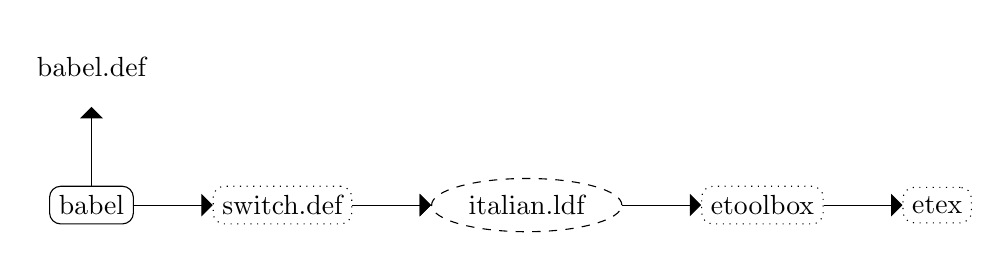
\begin{tikzpicture}
 \tikzset{main node/.style={rectangle, draw,
 		text centered, rounded corners}, }
 \tikzset{internal node/.style={rectangle, draw,dotted,
 		text centered, rounded corners}, }
 \tikzset{driver node/.style={ellipse, draw,dashed,
 		text centered}, }
 \tikzset{formato node/.style={rectangle, draw,dotted,
 		text centered}, }
 \tikzset{cfg node/.style={minimum size=1cm}, }
 \tikzset{linea/.style={-triangle 90},}
 \node[main node] (1) {babel};
 \node[internal node] (2)[right=of 1] {switch.def};

 \node[driver node] (3)[right =of 2] {italian.ldf};
 \node[internal node] (4)[right =of 3] {etoolbox};
 \node[cfg node] (5)[ above =of 1] {babel.def};
 \node[internal node] (6)[right =of 4] {etex};
 \foreach \x /\y in{1/2,2/3,2/3,3/4,1/5,4/6}
 \path[linea] (\x) edge node {} (\y);
% %% 
 \end{tikzpicture}
\end{document}